\documentclass[12pt]{article}
\usepackage{mathematics}

\begin{document}

\section*{Tower struts}

\begin{mdframed}
  A tower of base width $w$ and height $h$ is composed of two sides inclined towards each other at
  the same angle $\beta$. A series of diagonal struts at angle $\alpha < \beta$ join the two
  sides. The two sides of the tower do not meet at the top.

  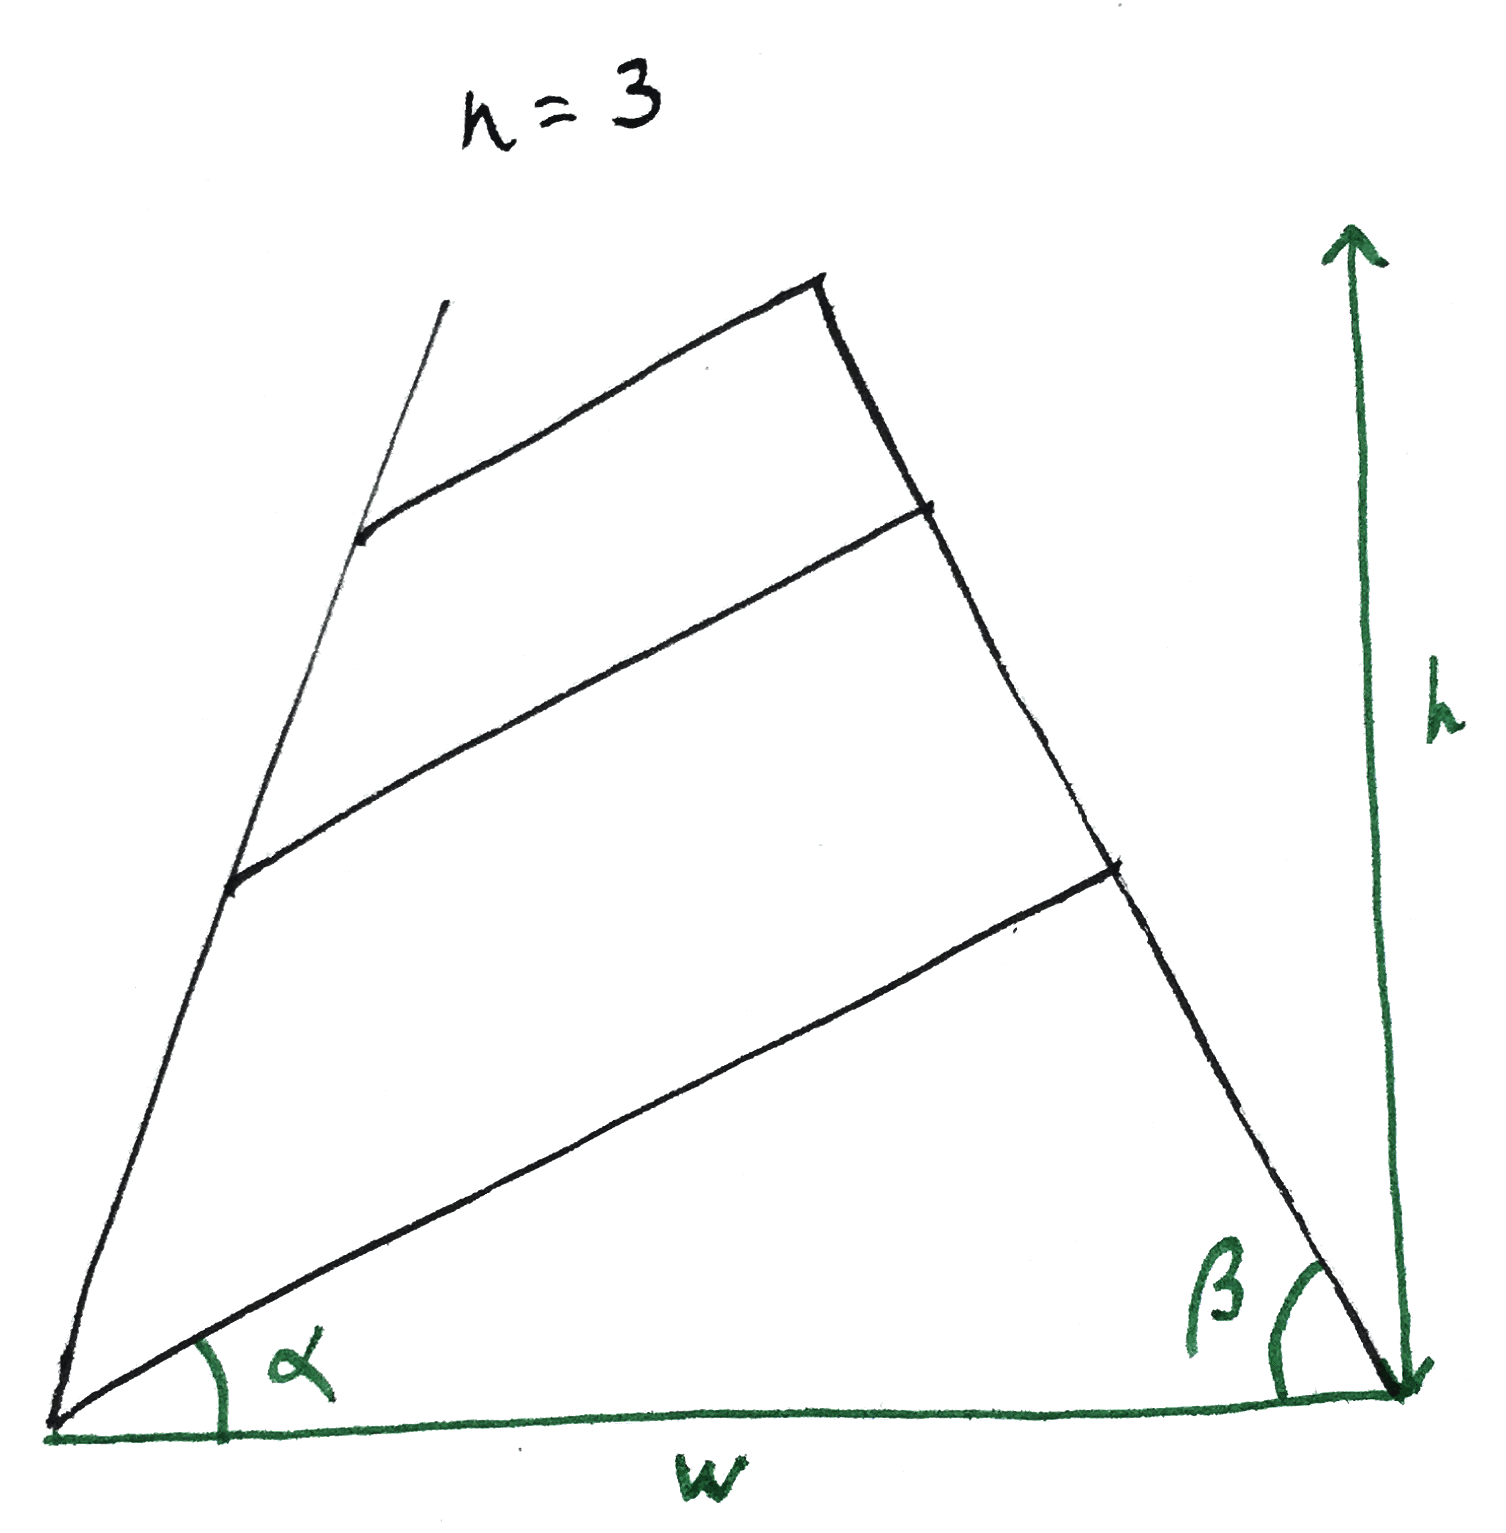
\includegraphics[width=200pt]{img/puzzles-tower-struts.png}

  There are $n$ diagonal struts, with the first strut starting at height 0 and the last strut
  ending at height $h$.

  $w, h, \beta$ and $n$ are given. What must $\alpha$ be?
\end{mdframed}
Let the origin be the bottom left hand corner of the tower.

Let $p = \frac{\tan\alpha}{\tan\alpha + \tan\beta}$ be the ratio of the two angles.

The first strut intersects the right side at a horizontal distance $pw$ from the origin.

Therefore the height of the intersection of the first strut is $pw\tan\alpha$.

Note that since the left and right sides are inclined at the same angle, the width of the tower at
the height of intersection of the first strut is $w - 2(1 - pw)$.


\section{n-omino}
\begin{mdframed}
  You have a $n$-omino. (Like a tetris piece but with arbitrarily many pieces.)
  Now pick two points with uniform distribution on that piece. Prove that the
  probability that the line between them is contained on the piece is of the
  form $p - q\ln(r)$ where $p,q$ and $r$ are rational.
\end{mdframed}
~\\

Assumptions:
\begin{enumerate}
\item A random $n$-omino is generated as follows: place a square tile at an
  arbitrary location in a plane; while the number of tiles is less than $n$,
  choose an edge uniformly from among the available edges and place a tile
  adjoining that edge.
\end{enumerate}

Define an ``internal'' line to be a line connecting two points on an $n$-omino
that is contained in the $n$-omino.

Let $\omega$ denote the desired probability that a line between two points
chosen uniformly on an $n$-omino is internal.

For $n=1$ and $n=2$ we have $\omega = 1$, since the only possible
configurations are rectangles, and these are convex polygons.

For $n=3$ the configuration is a rectangle with probability $\frac{1}{3}$ and
an L-shape with probability $\frac{2}{3}$. In the former case the line is
always internal. In the latter case, if the first point is in the corner
square, then the line is always internal; otherwise, the probability that the
line is internal is equal to the
\begin{align*}
  \omega = \frac{1}{3}\cdot 1 + \frac{2}{3} \Big(\text{random area enclosed by line through center}\Big)
\end{align*}

\section{IMO}

\newpage
\begin{mdframed}
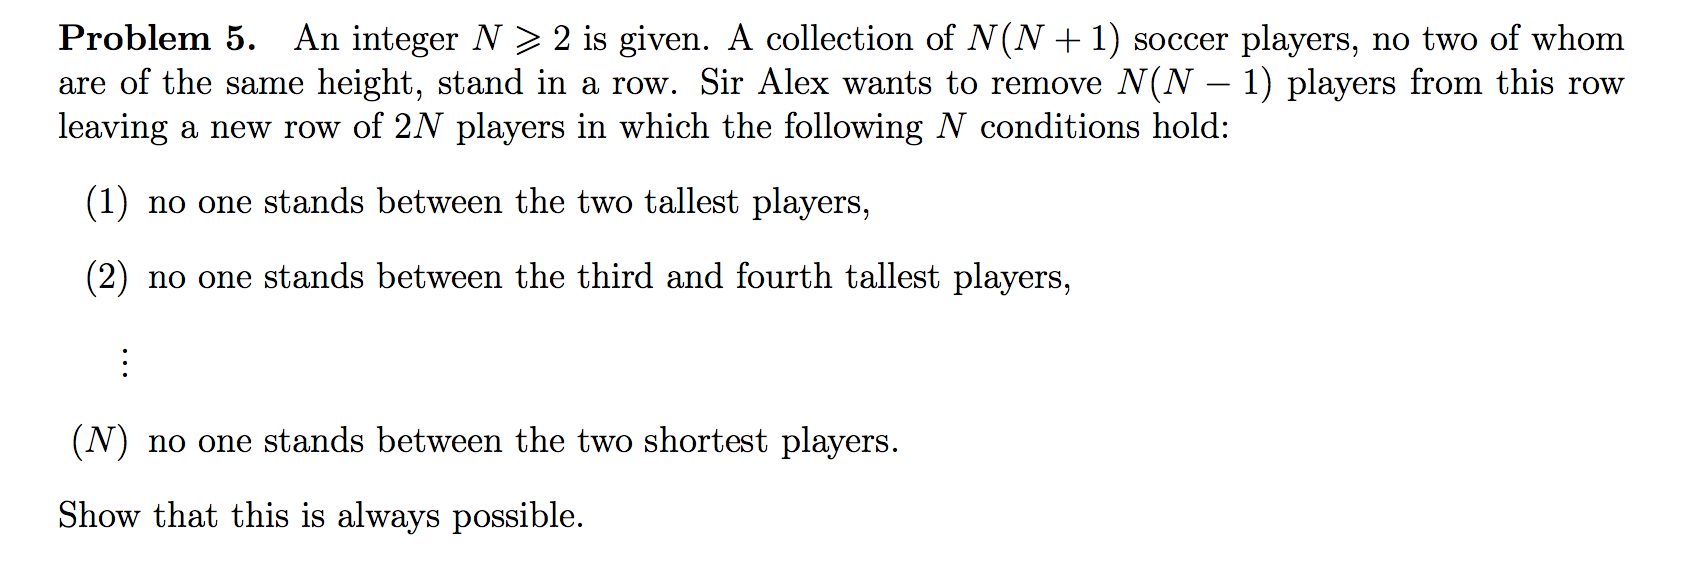
\includegraphics[width=400pt]{img/puzzles-imo-2017-5.png}
\end{mdframed}

\begin{enumerate}
\item Reverse direction: starting from a row of $2N$ satisfying the conditions, show that it is
  possible to generate an arbitrary superrow of $N(N+1)$ by inserting players?
\item Characterize the starting row as a permutation of $1, \ldots, N(N+1)$?

  Let $S_n$ be the set of permutations of $n$ objects.

  Let the starting row be $r \in S_{N(N+1)}$.

  Let $R_n \subset S_n$ be the subset of permutations of $n$ objects that satisfy the conditions.

  \begin{claim*}
    For all $\sigma \in S_{N(N+1)}$ there exists $\rho \in R_{2N}$ such that $\rho$ can be
    transformed into $\sigma$ via insertions.
  \end{claim*}

\item Formalize using a tuple of binary indicator variables $(e_1, e_2, \ldots, e_{N(N+1)})$, where
  $e_i \in \{0, 1\}$. Let $R_{N(N+1)}$ be the set of all possible starting rows and let $E_{N(N+1)}$
    be the set of all indicator tuples.

  Define the removal function
  $$f:R_{N(N+1)} \times E_{N(N+1)} \to R_{2N}$$
  and show for all $r \in R_{N(N+1)}$ there exists $e \in E_{N(N+1)}$ such that $f(r, e)$ satisfies
  the conditions?
\item Clearly the final number of players must be even, but what is the significance of the number
  $N(N+1)$?

\begin{verbatim}
|    |    <1 |     1 |     2 |     3 |     4 |
|----+-------+-------+-------+-------+-------|
| <1 | 12345 | 21345 | 23145 | 23415 | 23451 |
|  1 | 21345 | 12345 | 13245 | 13425 | 13452 |
|  2 | 31245 | 13245 | 12345 | 12435 | 12453 |
|  3 | 41235 | 14235 | 12435 | 12345 | 12354 |
|  4 | 51234 | 15234 | 12534 | 12354 | 12345 |
\end{verbatim}
\end{enumerate}

\newpage
\begin{mdframed}
   I pick ten points in the plane. I have ten coins.

   Show that I can cover all the points with the ten coins, with none of the coins overlapping.
\end{mdframed}

\begin{proof}
  Show (by identifying tiling region and using trigometry) that maximal packing of circles in plane
  covers just over $90\%$ of the plane.

  Therefore the expected number of points covered by exceeds 9.

  Therefore it is sokmetimes 10.
\end{proof}

\end{document}
